\subsection{Attitude Controller}
The attitude controller for the quadcopter is designed using a state space representation of the system. This helps handling the coupled angular response of the quadcopter. The chosen states for the system are the three angular positions and the three angular velocities. The input vector of the attitude system consists of the four motor rotational speeds and the output vector consists of the three angles, roll, pitch and yaw. Below, the state, input and output vectors are seen as.
%
\begin{flalign}
	\vec{x}(t)&= 
	\begin{bmatrix}
		\phi & \theta & \psi & \dot{\phi} &	\dot{\theta} & \dot{\psi} 
	\end{bmatrix}	\nonumber
	^T\\
	\vec{y}(t)&= 
	\begin{bmatrix}
		\phi &	\theta & \psi 
	\end{bmatrix}	\nonumber
	^T\\
	\vec{u}(t)&= 
	\begin{bmatrix}
		\omega_1 & \omega_2 &	\omega_3 &	\omega_4 
	\end{bmatrix}\nonumber	
	^T \ .
\end{flalign}

The vectors above are then used in construction of the state space matrix representation as
\begin{flalign}
	\vec{\dot{x}}(t)&=\vec{A} \ \vec{x}(t) + \vec{B} \ \vec{u}(t)
	\label{xDotSS} 
\end{flalign}
\vspace{-0.9 cm}
\begin{flalign}
	\vec{y}(t)&=\vec{C} \ \vec{x}(t) + \vec{D} \ \vec{u}(t)\label{ySS} 
\end{flalign}
%
where $\vec{A}$ is the system matrix, $\vec{B}$ is the input matrix, $\vec{C}$ is the output matrix and $\vec{D}$ is the feedback matrix.

The values for the $\vec{A}$, $\vec{B}$, $\vec{C}$ and $\vec{D}$ matrices are obtained from the linearized attitude equations, yielding the matrices shown below. As $\vec{D}$ is a zero matrix, only $\vec{A}$, $\vec{B}$ and $\vec{C}$ are shown. 

\footnotesize{
\begin{flalign}   \label{Amatrix}
	\vec{A}=
	\begin{bmatrix}
		\ 0 & 0 & 0 & 1 & 0 & 0     \ \ \ \\ 
		\ 0 & 0 & 0 & 0 & 1 & 0     \ \ \ \\ 
		\ 0 & 0 & 0 & 0 & 0 & 1     \ \ \ \\
		\ 0 & 0 & 0 & 0 & 0 & 0     \ \ \ \\ 
		\ 0 & 0 & 0 & 0 & 0 & 0     \ \ \ \\ 
		\ 0 & 0 & 0 & 0 & 0 & 0     \ \ \  
	\end{bmatrix}\nonumber
\end{flalign} \label{Bmatrix}
\vspace{-0.3 cm}
\begin{flalign}
    \vec{B} =
	\begin{bmatrix}
		\ 0 & 0 & 0 & 0      \ \ \ \\ 
		\ 0 & 0 & 0 & 0      \ \ \ \\ 
		\ 0 & 0 & 0 & 0      \ \ \ \\
		\ 0 & \si{-\frac{2  k_{\mathrm{th}} L \overline{\omega}_2}{J_x}} & 0 & \si{\frac{2 k_{\mathrm{th}}  L \overline{\omega}_4}{J_x}}      \ \ \ \\ 
		\ \si{\frac{2 k_{\mathrm{th}} L  \overline{\omega}_1}{J_y}} & 0 & \si{-\frac{2  k_{\mathrm{th}} L \overline{\omega}_3}{J_y}} & 0      \ \ \ \\ 
		\ \frac{2 k_{\mathrm{d}} {\overline{\omega}_1}}{J_z} & - \frac{2 k_{\mathrm{d}} {\overline{\omega}_2}}{J_z} & \frac{2 k_{\mathrm{d}}  {\overline{\omega}_3}}{J_z} & - \frac{2 k_{\mathrm{d}} {\overline{\omega}_4}}{J_z}      \ \ \ 		
	\end{bmatrix}\nonumber
\end{flalign}
\vspace{-0.3 cm}
\begin{flalign} \label{Cmatrix}
	\vec{C} =	 
	\begin{bmatrix}
		\ 1 & 0 & 0 & 0 & 0 & 0     \ \ \ \\ 
		\ 0 & 1 & 0 & 0 & 0 & 0     \ \ \ \\ 
		\ 0 & 0 & 1 & 0 & 0 & 0     \ \ \ 
	\end{bmatrix}\nonumber
\end{flalign} }
\normalsize
The attitude control is based on a state feedback and an integral term in order to be able to track a given reference. As not all states are measured a reduced order observer is implemented to estimate the angular velocities of the quadcopter. Due to the separation principle, both subsystems can be designed independently. \cite{ssReference}
\\
\\
\noindent\autoref{AttitudeControlDiagram} shows how these designs are related.
\begin{figure}[H]
    \centering
    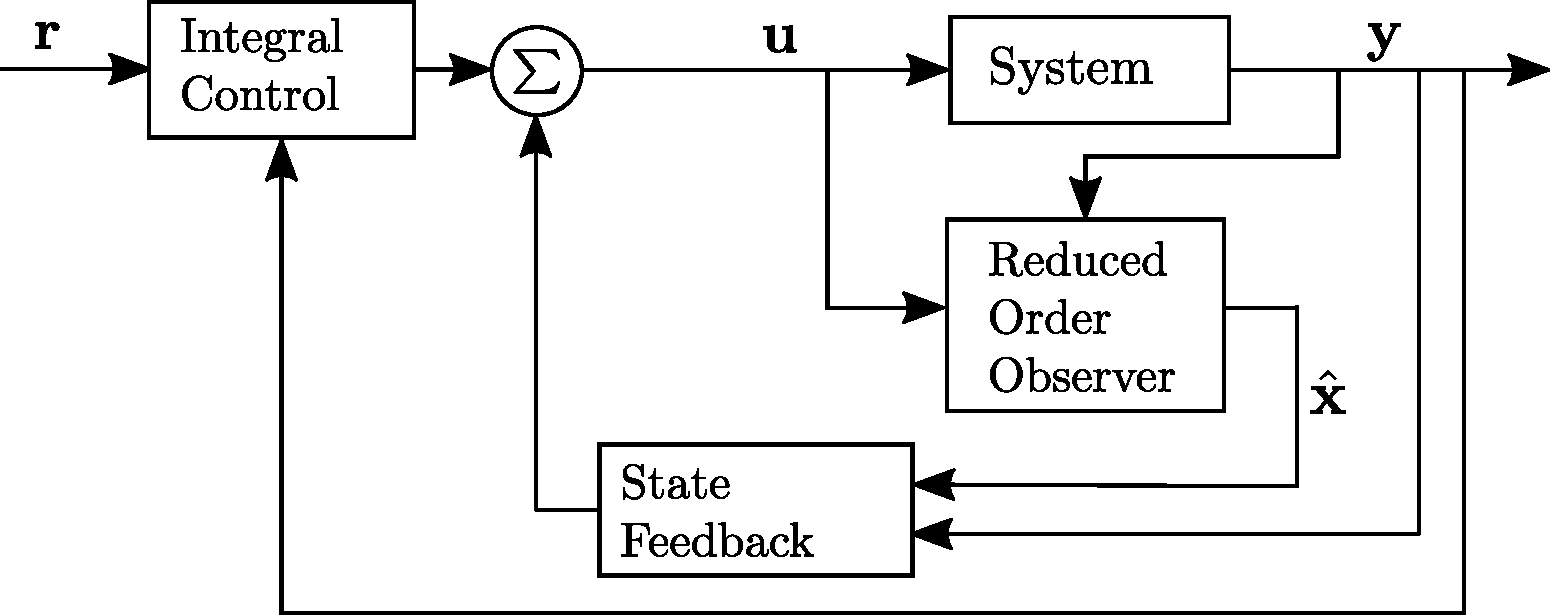
\includegraphics[scale=0.25]{figures/AttitudeControlDiagram}
    \caption{ Control structure for the system, including the state feedback, the integral controller and the reduced order observer.}
    \label{AttitudeControlDiagram}
\end{figure}

%--------------------- StateFeedback with Integral Control ----------------------------
The design of the state feedback and integral control is shown in \autoref{fig:DetailedControllerColorDiagram}.
\begin{figure}[H]
    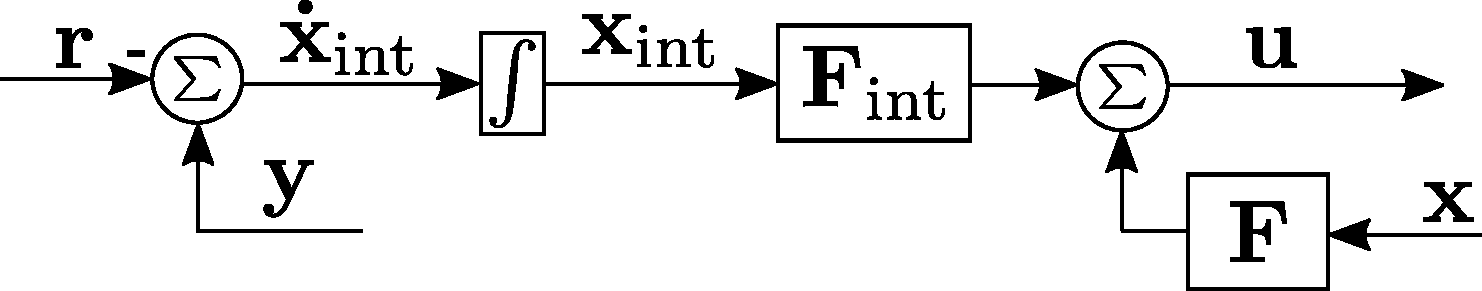
\includegraphics[scale=.3]{figures/DetailedControllerColorDiagram}
    \centering
    \captionof{figure}{State feedback and integral controller in the attitude control structure.}
    \label{fig:DetailedControllerColorDiagram}
\end{figure}
As there are three outputs to track, three states, $\vec{x}_{\mathrm{int}}(t)$, are added to the already existing state vector. This leads to the extended system
%
\begin{flalign} 
\dot{\vec{x}}_\mathrm{e}(t) &= \vec{A}_\mathrm{e} \  \vec{x}_\mathrm{e}(t) + \vec{B}_\mathrm{e} \  \vec{u}(t) + 
\begin{bmatrix}
\ \vec{0}     \ \ \ \\ 
\ \vec{-I}     \ \ \  		
\end{bmatrix}
\vec{r}(t) 
\label{xdotSSExtended}\\ 
\vec{y}(t) &= \vec{C}_\mathrm{e} \  \vec{x}_\mathrm{e} 
\label{ySSExtended}
\end{flalign} 
%
where\\
\scriptsize{
\begin{minipage}{0.28\linewidth}
    \begin{flalign}
    \dot{\vec{x}}_\mathrm{e}(t)= 
    \begin{bmatrix}
    \ \dot{\vec{x}}(t)      \ \  \\ 
    \ \dot{\vec{x}}_{\mathrm{int}}(t)      \ \   		
    \end{bmatrix} \nonumber
    \end{flalign}
\end{minipage}\hfill
\begin{minipage}{0.2\linewidth}
    \begin{flalign}
    \vec{A}_\mathrm{e}=
    \begin{bmatrix}
    \ \vec{A}  & \vec{0}    \ \  \\ 
    \ \vec{C}  & \vec{0}    \ \   		
    \end{bmatrix} \nonumber
    \end{flalign}
\end{minipage}   \hfill 
\begin{minipage}{0.2\linewidth}
    \begin{flalign}
    \vec{B}_\mathrm{e}=
    \begin{bmatrix}
    \ \vec{B}    \ \  \\ 
    \ \vec{0}     \ \   		
    \end{bmatrix} \nonumber
    \end{flalign}
\end{minipage}\hfill
\begin{minipage}{0.2\linewidth}
    \begin{flalign}
    \vec{C}_\mathrm{e}=
    \begin{bmatrix}
    \ \vec{C}  & \vec{0}  \ \   		
    \end{bmatrix} \nonumber
    \end{flalign}
\end{minipage} }
\\
\normalsize

The feedback law for this design approach is given by \eqref{eq:ssControllerAction}. Its design is done as a conventional state feedback, where the goal is to choose an appropriate $\vec{F}_\mathrm{e}=[\vec{F} \ \vec{F}_{\mathrm{int}}]$ matrix, such that the eigenvalues of $\vec{A}_\mathrm{e}+\vec{B}_\mathrm{e}\vec{F}_\mathrm{e}$ are the closed loop poles giving the desired dynamics.
%
\begin{flalign} 
    \vec{u}(t) &=\vec{F} \  \vec{x}(t) + \ \vec{F}_{\mathrm{int}} \  \vec{x}_{\mathrm{int}}(t)
    \label{eq:ssControllerAction}
\end{flalign}
%
Once $\vec{F}_\mathrm{e}$ is obtained, it is split into $F$ and $F_{\mathrm{int}}$. In this way, the controller is implemented as shown in \autoref{fig:DetailedControllerColorDiagram}.\\

%--------------------- Reduced-Order Observer ----------------------------

Since certain states in the system are not measured, an observer estimates the remaining states by means of the system output and input. With this approach, the first three states, $\vec{x}_{1:3}$, are equal to the outputs, $\vec{y}$, whereas the other three states, $\vec{x}_{4:6}$, are estimated as $\hat{\vec{x}}_{4:6}$.

The observer is designed by finding the matrix $\vec{L}_{\mathrm{obs}}$ such that the eigenvalues of the matrix $\vec{A}_{22}+\vec{L}_{\mathrm{obs}}\ \vec{A}_{12}$ \cite{ssReference}. This is done splitting the original system matrices into submatrices, as seen below\\
%
\begin{minipage}{0.45\linewidth}
    \begin{flalign}
    \vec{A}=
    \begin{bmatrix}
    \ \vec{A}_{11}  & \vec{A}_{12}    \ \ \ \\ 
    \ \vec{A}_{21}  & \vec{A}_{22}    \ \ \  		
    \end{bmatrix} \nonumber
    \end{flalign}
\end{minipage}   \hfill 
\begin{minipage}{0.45\linewidth}
    \begin{flalign}
    \vec{B}=
    \begin{bmatrix}
    \ \vec{B}_1    \ \ \ \\ 
    \ \vec{B}_2     \ \ \  		
    \end{bmatrix} \ . \nonumber
    \end{flalign}
\end{minipage}\\
\normalsize

With the observer matrix, the observer equation is derived. See \eqref{eq:eqobservertheorem}. This ensures an estimate $\hat{\vec{x}}_{4:6}$ which converges to $\vec{x}_{4:6}$ at a rate given by the chosen observer poles.
\small{
\begin{flalign}
    \vec{\hat{\dot{x}}}_{4:6} &= \vec{A}_{21}\vec{y} + \vec{A}_{22}\vec{\hat{x}}_{4:6} + \vec{B_2} + \vec{L}_{\mathrm{obs}}\vec{(A}_{12}\vec{\hat{x}}_{4:6} - \vec{A}_{21}\vec{x}_{4:6}) \label{eq:eqobservertheorem}
\end{flalign}
\normalsize
\\
This estimation of $\vec{x}_{4:6}$ is also seen in \autoref{fig:observerDiagram}.

\begin{figure}[H]
    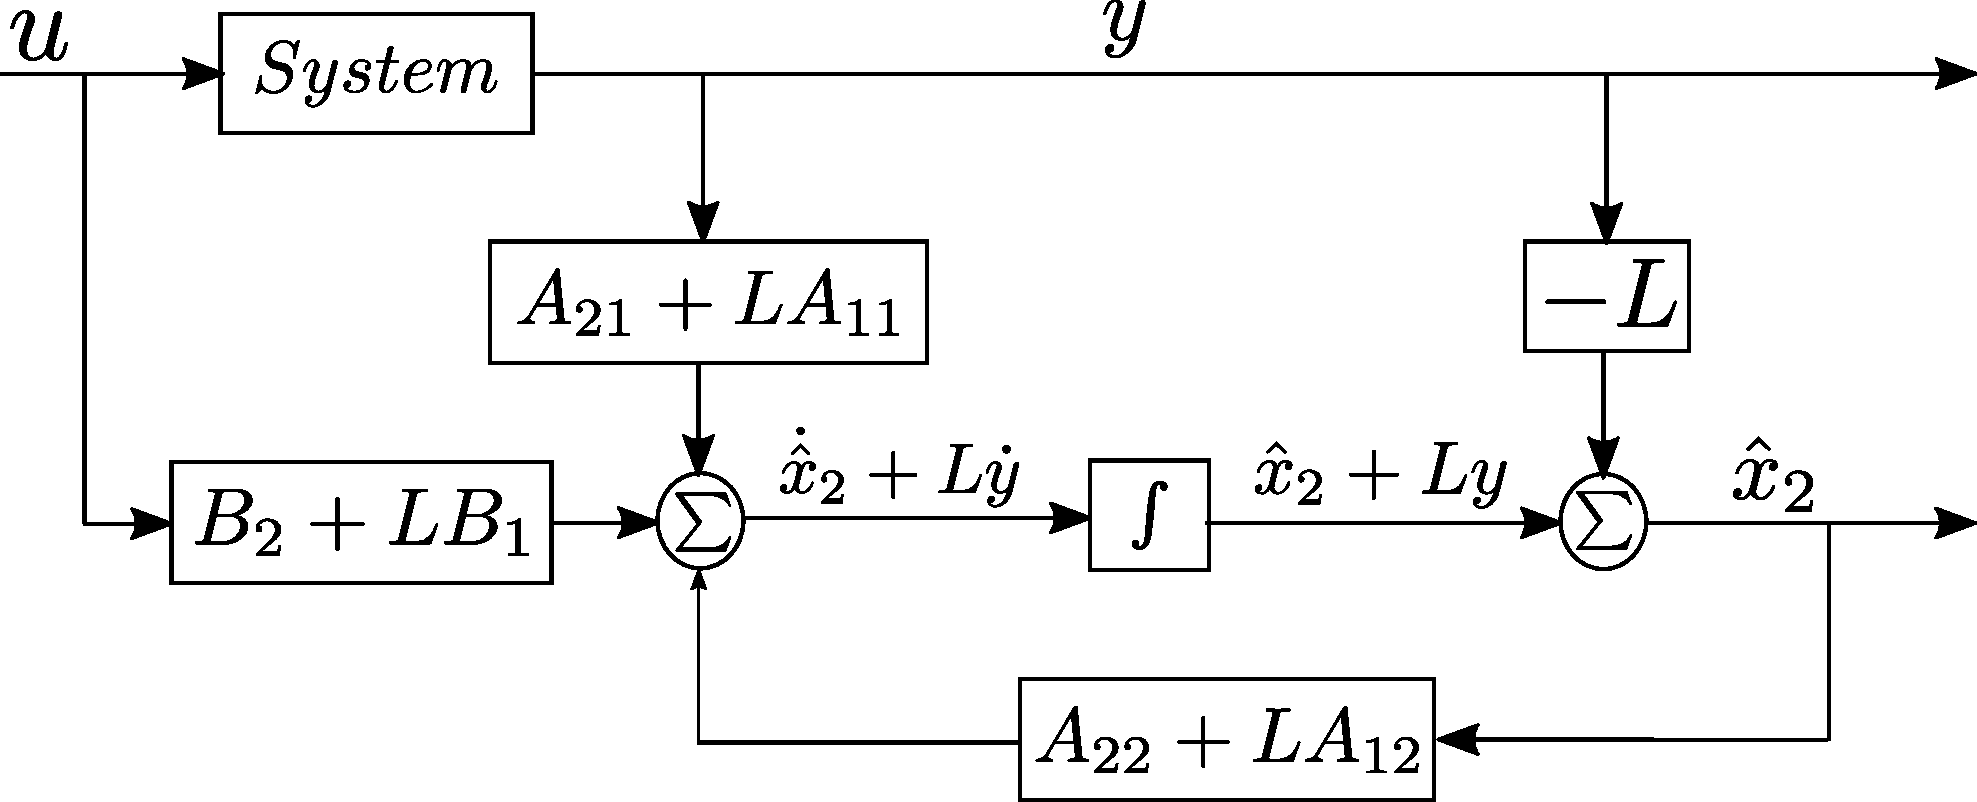
\includegraphics[scale=.15]{figures/observerDiagram}
    \centering
    \captionsetup{justification=centering}
    \captionof{figure}{Detailed diagram of the reduced order observer that shows its implementation.}
    \label{fig:observerDiagram}
\end{figure}